% Generated by research/scripts/tables.py -- do not edit by hand.
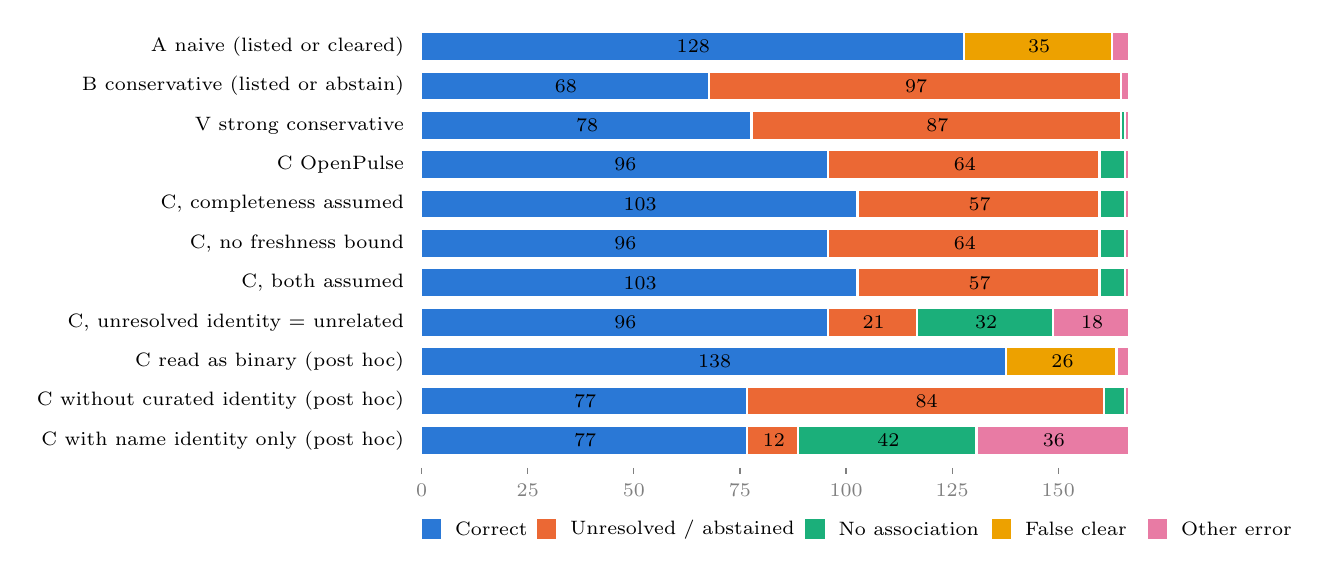
\begin{tikzpicture}[font=\scriptsize]
\definecolor{opcorrect}{HTML}{2A78D6}
\definecolor{opunresolved}{HTML}{EB6834}
\definecolor{opnoassociation}{HTML}{1BAF7A}
\definecolor{opfalseclear}{HTML}{EDA100}
\definecolor{opothererror}{HTML}{E87BA4}
\node[anchor=east] at (-0.1,-0.00) {A naive (listed or cleared)};
\fill[opcorrect] (0.000,-0.17) rectangle (6.868,0.17);
\node at (3.449,-0.00) {128};
\fill[opfalseclear] (6.898,-0.17) rectangle (8.754,0.17);
\node at (7.841,-0.00) {35};
\fill[opothererror] (8.784,-0.17) rectangle (8.970,0.17);
\node[anchor=east] at (-0.1,-0.50) {B conservative (listed or abstain)};
\fill[opcorrect] (0.000,-0.67) rectangle (3.635,-0.33);
\node at (1.832,-0.50) {68};
\fill[opunresolved] (3.665,-0.67) rectangle (8.862,-0.33);
\node at (6.278,-0.50) {97};
\fill[opothererror] (8.892,-0.67) rectangle (8.970,-0.33);
\node[anchor=east] at (-0.1,-1.00) {V strong conservative};
\fill[opcorrect] (0.000,-1.17) rectangle (4.174,-0.83);
\node at (2.102,-1.00) {78};
\fill[opunresolved] (4.204,-1.17) rectangle (8.862,-0.83);
\node at (6.548,-1.00) {87};
\fill[opnoassociation] (8.892,-1.17) rectangle (8.916,-0.83);
\fill[opothererror] (8.946,-1.17) rectangle (8.970,-0.83);
\node[anchor=east] at (-0.1,-1.50) {C OpenPulse};
\fill[opcorrect] (0.000,-1.67) rectangle (5.144,-1.33);
\node at (2.587,-1.50) {96};
\fill[opunresolved] (5.174,-1.67) rectangle (8.593,-1.33);
\node at (6.898,-1.50) {64};
\fill[opnoassociation] (8.623,-1.67) rectangle (8.916,-1.33);
\fill[opothererror] (8.946,-1.67) rectangle (8.970,-1.33);
\node[anchor=east] at (-0.1,-2.00) {C, completeness assumed};
\fill[opcorrect] (0.000,-2.17) rectangle (5.521,-1.83);
\node at (2.775,-2.00) {103};
\fill[opunresolved] (5.551,-2.17) rectangle (8.593,-1.83);
\node at (7.087,-2.00) {57};
\fill[opnoassociation] (8.623,-2.17) rectangle (8.916,-1.83);
\fill[opothererror] (8.946,-2.17) rectangle (8.970,-1.83);
\node[anchor=east] at (-0.1,-2.50) {C, no freshness bound};
\fill[opcorrect] (0.000,-2.67) rectangle (5.144,-2.33);
\node at (2.587,-2.50) {96};
\fill[opunresolved] (5.174,-2.67) rectangle (8.593,-2.33);
\node at (6.898,-2.50) {64};
\fill[opnoassociation] (8.623,-2.67) rectangle (8.916,-2.33);
\fill[opothererror] (8.946,-2.67) rectangle (8.970,-2.33);
\node[anchor=east] at (-0.1,-3.00) {C, both assumed};
\fill[opcorrect] (0.000,-3.17) rectangle (5.521,-2.83);
\node at (2.775,-3.00) {103};
\fill[opunresolved] (5.551,-3.17) rectangle (8.593,-2.83);
\node at (7.087,-3.00) {57};
\fill[opnoassociation] (8.623,-3.17) rectangle (8.916,-2.83);
\fill[opothererror] (8.946,-3.17) rectangle (8.970,-2.83);
\node[anchor=east] at (-0.1,-3.50) {C, unresolved identity = unrelated};
\fill[opcorrect] (0.000,-3.67) rectangle (5.144,-3.33);
\node at (2.587,-3.50) {96};
\fill[opunresolved] (5.174,-3.67) rectangle (6.275,-3.33);
\node at (5.740,-3.50) {21};
\fill[opnoassociation] (6.305,-3.67) rectangle (8.000,-3.33);
\node at (7.168,-3.50) {32};
\fill[opothererror] (8.030,-3.67) rectangle (8.970,-3.33);
\node at (8.515,-3.50) {18};
\node[anchor=east] at (-0.1,-4.00) {C read as binary (post hoc)};
\fill[opcorrect] (0.000,-4.17) rectangle (7.407,-3.83);
\node at (3.719,-4.00) {138};
\fill[opfalseclear] (7.437,-4.17) rectangle (8.808,-3.83);
\node at (8.138,-4.00) {26};
\fill[opothererror] (8.838,-4.17) rectangle (8.970,-3.83);
\node[anchor=east] at (-0.1,-4.50) {C without curated identity (post hoc)};
\fill[opcorrect] (0.000,-4.67) rectangle (4.120,-4.33);
\node at (2.075,-4.50) {77};
\fill[opunresolved] (4.150,-4.67) rectangle (8.647,-4.33);
\node at (6.413,-4.50) {84};
\fill[opnoassociation] (8.677,-4.67) rectangle (8.916,-4.33);
\fill[opothererror] (8.946,-4.67) rectangle (8.970,-4.33);
\node[anchor=east] at (-0.1,-5.00) {C with name identity only (post hoc)};
\fill[opcorrect] (0.000,-5.17) rectangle (4.120,-4.83);
\node at (2.075,-5.00) {77};
\fill[opunresolved] (4.150,-5.17) rectangle (4.766,-4.83);
\node at (4.473,-5.00) {12};
\fill[opnoassociation] (4.796,-5.17) rectangle (7.030,-4.83);
\node at (5.928,-5.00) {42};
\fill[opothererror] (7.060,-5.17) rectangle (8.970,-4.83);
\node at (8.030,-5.00) {36};
\draw[gray] (0.000,-5.35) -- ++(0,-0.08) node[below] {0};
\draw[gray] (1.347,-5.35) -- ++(0,-0.08) node[below] {25};
\draw[gray] (2.695,-5.35) -- ++(0,-0.08) node[below] {50};
\draw[gray] (4.042,-5.35) -- ++(0,-0.08) node[below] {75};
\draw[gray] (5.389,-5.35) -- ++(0,-0.08) node[below] {100};
\draw[gray] (6.737,-5.35) -- ++(0,-0.08) node[below] {125};
\draw[gray] (8.084,-5.35) -- ++(0,-0.08) node[below] {150};
\fill[opcorrect] (0.00,-6.25) rectangle ++(0.25,0.25);
\node[anchor=west] at (0.30,-6.13) {Correct};
\fill[opunresolved] (1.46,-6.25) rectangle ++(0.25,0.25);
\node[anchor=west] at (1.76,-6.13) {Unresolved / abstained};
\fill[opnoassociation] (4.87,-6.25) rectangle ++(0.25,0.25);
\node[anchor=west] at (5.17,-6.13) {No association};
\fill[opfalseclear] (7.24,-6.25) rectangle ++(0.25,0.25);
\node[anchor=west] at (7.54,-6.13) {False clear};
\fill[opothererror] (9.22,-6.25) rectangle ++(0.25,0.25);
\node[anchor=west] at (9.52,-6.13) {Other error};
\end{tikzpicture}
